\documentclass{beamer}

\usepackage {color}
\usepackage{graphicx}

%COLORS
\definecolor{mcYellow}{RGB}{255, 195, 0}
\definecolor{mcRed}{RGB}{221, 16, 33}

\title{\textbf{\color{mcRed}\underline{A Simple Approach to LaTeX}}}
\subtitle{*A Windows based tutorial*}

\begin{document}
    \author{
        \begin{center}
        By,\\
      Kevin Olofson,\\
      \and
      Derek Vanden-Bulcke,\\
      \and
And\\
      Nicole Korb\\
      \end{center}
    }

    \setbeamercolor{background canvas}{bg=mcYellow}

	\frame {
        \date{}
		\titlepage
	}
	\frame {
		\frametitle{Setting Up LaTeX}
        \begin{center}%centers
            \textbf{\color{mcRed}\underline{After all Required Software Installations:}}
            \begin{itemize}
    			\item Open WinEdt
    			\item Create a new .tex File
                \item Save it somewhere you can find it
    		\end{itemize}
        \color{black}\textbf{Now you're ready to start creating your document!}
		\end{center} %centers
	}
    \frame {
        \frametitle{Let's Start Coding!}
        \begin{center}
            \textbf{\color{mcRed}\underline{For the Very First Few Lines of Code We Will Add:}}
            \begin{figure}
                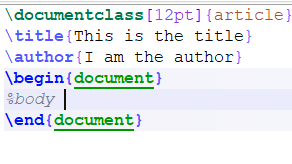
\includegraphics[width=\linewidth]{img_1.png}
            \end{figure}
        \end{center}
    }
    \frame {
        \frametitle{Breaking Down the Code}
        \begin{center}
            \textbf{\color{mcRed}\underline{Lets Break down and define each line we just added:}}
            \color{black}\\Line 1 Creates the type of document we are creating such as:
            \begin{itemize}
              \item beamer, for Presentations
              \item article, for Papers
              \item etc.
            \end{itemize}
            \color{black}Line 2 Creates the title \\Line 3 Creates the Author
            \\However, the next two lines are the most important! Everything we want on our document we will place in between those two lines!
        \end{center}
    }
    \begin{frame} [fragile]
        \frametitle{The Basics 1/3}
        \begin{center}
            \textbf{\color{mcRed}\underline{Adding Text:}}
            \begin{verbatim}
                \documentclass[12pt]{article}
                \begin{document}
                \maketitle
            \end{verbatim}
            \textit{To add some text just type!}
            \begin{verbatim}
                \end{document}
            \end{verbatim}
        \end{center}
    \end{frame}
    \begin{frame} [fragile]
        \frametitle{The Basics 2/3}
        \begin{center}
            \textbf{\color{mcRed}\underline{Adding Color:}}
            \color{black}\\To Add Color to Text:
            \\First you must import package 
            \begin{verbatim}
                \usepackage{color}
                 color{addcolorhere}
            \end{verbatim}
            \textbf{To Add a Custom Color to Text:}
        \begin{verbatim}
            \definecolor{myColor}{RGB}{221, 16, 33}
            \color{myColor}Hello World!
        \end{verbatim}
            \textbf{To Add Color to the background:}
    \begin{verbatim}
            \pagecolor{colorhere}
    \end{verbatim}
        \end{center}
    \end{frame}
    \begin{frame} [fragile]
        \frametitle{The Basics 3/3}
        \begin{center}
            \textbf{\color{mcRed}\underline{Styling Text:}}
                \item \underline{Italics}
                \begin{verbatim}
                    \textit{text}
                \end{verbatim}
                \item \underline{Bold}
                \begin{verbatim}
                    \textbf{text}
                \end{verbatim}
                \item \underline{Boxing}
                \begin{verbatim}
                    \framebox{text}
                \end{verbatim}
        \end{center}
    \end{frame}
    \begin{frame} [fragile]
        \frametitle{More LaTeX Knowledge}
        \begin{center}
            \textbf{\color{mcRed}\underline{Fun LaTeX Syntax:}}
            \begin{itemize}
              \item Adding a new line
              \begin{verbatim}
                \\this makes me go on a new line
              \end{verbatim}
              \item Centering Text
              \begin{verbatim}
                \begin{center}
                    %Anything here will get centered!
                \end{center}
              \end{verbatim}
              \item Adding Bullets
                \begin{verbatim}
                    \begin{itemize}
                        \item I'M first!
                    \end{itemize}
                \end{verbatim}
              \end{itemize}
        \end{center}
    \end{frame}
    \frame {
        \frametitle{Conclusion}
        \begin{center}
            \textbf{\color{mcRed}\underline{Congratulations!}}
            \\Now That you have the basics go start coding your first document!
        \end{center}
    }
\end{document} 